%% LyX 2.3.4.3 created this file.  For more info, see http://www.lyx.org/.
%% Do not edit unless you really know what you are doing.
\documentclass[10pt,english,brazil]{beamer}
\usepackage[T1]{fontenc}
\usepackage[utf8]{inputenc}
\setcounter{secnumdepth}{3}
\setcounter{tocdepth}{3}
\usepackage{amsthm}
\usepackage{graphicx}
\usepackage[numbers]{natbib}
\PassOptionsToPackage{normalem}{ulem}
\usepackage{ulem}

\makeatletter
%%%%%%%%%%%%%%%%%%%%%%%%%%%%%% Textclass specific LaTeX commands.
% this default might be overridden by plain title style
\newcommand\makebeamertitle{\frame{\maketitle}}%
% (ERT) argument for the TOC
\AtBeginDocument{%
  \let\origtableofcontents=\tableofcontents
  \def\tableofcontents{\@ifnextchar[{\origtableofcontents}{\gobbletableofcontents}}
  \def\gobbletableofcontents#1{\origtableofcontents}
}
\theoremstyle{definition}
\newtheorem*{example*}{\protect\examplename}

%%%%%%%%%%%%%%%%%%%%%%%%%%%%%% User specified LaTeX commands.
\usetheme{Warsaw}
\newtheorem{thm}{Teorema}[]
\newtheorem{cor}[]{Corollary}
\newtheorem{lem}[]{Lema}
\newtheorem{prop}[]{Proposi\c{c}\~ao}
\theoremstyle{definition}
\newtheorem{defn}[]{Definition}
\theoremstyle{remark}
\newtheorem{rem}[thm]{Remark}
\usepackage{amsthm}\usepackage{amsfonts}

\makeatother

\usepackage{babel}
\addto\captionsbrazil{\renewcommand{\examplename}{Exemplo}}
\addto\captionsenglish{\renewcommand{\examplename}{Example}}
\providecommand{\examplename}{Exemplo}

\begin{document}
\title{\selectlanguage{english}%
Métodos Estatísticos Básicos}
\subtitle{Aula 8 - Análise combinatória}
\author{\selectlanguage{english}%
Prof. Regis Augusto Ely}
\institute{\selectlanguage{english}%
Departamento de Economia\\
Universidade Federal de Pelotas (UFPel)}
\date{\selectlanguage{english}%
Maio de 2014}
\makebeamertitle
\selectlanguage{brazil}%
\begin{frame}{Número de elementos do espaço amostral}

\begin{itemize}
\item A definição clássica de probabilidade requer que saibamos calcular
o número de elementos de determinados conjuntos.
\item Dividindo o número de elementos do espaço amostral que são favoráveis
a um evento A qualquer pelo número total de elementos do espaço amostral,
obtemos a probabilidade do evento A ocorrer (P(A)).
\item Lembrar de que esta definição clássica de probabilidade serve apenas
para espaços amostrais finitos e quando os resultados do experimento
são igualmente verossímeis.
\item Veremos cinco principais técnicas de enumeração de conjuntos, que
consistem em identificar quantos são os possíveis resultados de um
procedimento (experimento).
\end{itemize}
\end{frame}

\begin{frame}{Regra da multiplicação}

\begin{itemize}
\item \textbf{Quando se aplica a regra da multiplicação?} Se existirem k
procedimentos independentes e o k-ésimo procedimento puder ser executado
de $n_{i}$ maneiras, então o número total de maneiras de se executar
os k procedimentos é $n_{1}.n_{2}....n_{k}$.
\item É essencial que os procedimentos sejam independentes, ou seja, as
maneiras de executar um procedimento i não impactam nas maneiras de
executar outro procedimento j.
\item Os procedimentos podem ser interpretados como sendo sequenciais.
\end{itemize}
\end{frame}

\begin{frame}{Regra da multiplicação}

\begin{example*}
Uma peça passa por 2 estações de controle. Na primeira, 4 classificações
são possíveis (A, B, C, D). Na segunda estação, 3 classificações são
possíveis (X, Y, Z). Existem 3.4=12 possíveis classificações para
cada peça.
\end{example*}
\begin{center}
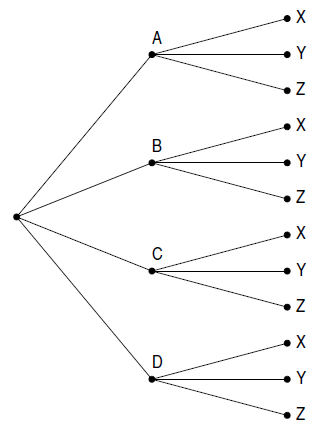
\includegraphics[scale=0.4]{sequencia}
\par\end{center}

\end{frame}

\begin{frame}{Regra da adição}

\begin{itemize}
\item \textbf{Quando se aplica a regra da adição?} Se existirem k procedimentos
independentes a serem realizados e o k-ésimo procedimento puder ser
executado de $n_{i}$ maneiras, então o número total de maneiras de
se executar os k procedimentos é $n_{1}+n_{2}+...+n_{k}.$
\item Note que agora não podemos executar 2 ou mais procedimentos em conjunto
(apenas um deles é possível).
\item Os procedimentos podem ser interpretados como sendo estáticos, em
apenas um período de tempo.
\end{itemize}
\begin{example*}
Se viajamos por ônibus ou trem, sendo que há 3 rodovias e 2 ferrovias,
o número possível de caminhos é $3+2=5$.
\end{example*}
\end{frame}

\begin{frame}{Permutações}

\begin{itemize}
\item \textbf{Fatorial: }sendo n um número inteiro positivo, definimos $n!=(n).(n-1).(n-2).....1$
como o fatorial de n. Também definimos $0!=1$.
\item \textbf{Permutação:} se tivermos n objetos, $_{n}P_{n}=n!$ será o
número de maneiras diferentes que podemos dispor esses objetos.
\item Note que este experimento pode ser interpretado como sequencial, mas
agora as etapas não são independentes, pois elas são as mesmas em
cada período de tempo. Além disso, estamos realizando o experimento
sem reposição (não podemos repetir um procedimento que já foi realizado).
\end{itemize}
\begin{example*}
Se tivermos três letras (a, b, c), temos as seguintes permutações:
abc, acb, bac, bca, cab, cba. Logo, como $n=3$, temos $_{3}P_{3}=3!=6$.
\end{example*}
\end{frame}

\begin{frame}{Arranjos}

\begin{itemize}
\item \textbf{Arranjos:} se, dados n objetos, queremos escolher r deles,
com $0\leq r\leq n$, e permutar os r escolhidos, denotamos por $nAr$
o número de maneiras de fazer isso, que é $nAr=\frac{n!}{(n-r)!}.$
\item Note que estamos calculando o número de permutação dos n objetos e
descontando o número de permutações dos (n-r) objetos restantes. Assim,
temos as permutações possíveis de n objetos ordenados r a r.
\end{itemize}
\begin{example*}
Se tivermos quatro letras (a, b, c, d), e queremos rearranjá-las de
2 em 2, temos as seguintes combinações, $_{4}A_{2}=\cfrac{4!}{(4-2)!}=12.$
\end{example*}
\end{frame}

\begin{frame}{Combinações}

\begin{itemize}
\item \textbf{Combinações:} se, dados n objetos, queremos escolher r deles,
com $0\leq r\leq n$, e permutar os r escolhidos, mas não nos importa
a ordem deles, então $C=\frac{n!}{r!(n-r)!}=\binom{n}{r}$.
\end{itemize}
\begin{example*}
se temos a, b, c e d, e $r=2$, então desejamos contar ab, ac, ad,
bc, bd, cd (não consideramos ba, ca, da, cb, db, dc). Ao todo são
$C=\frac{4!}{2!(4-2)!}=\binom{4}{2}=6$ combinações.
\end{example*}
\begin{itemize}
\item Note que uma vez que r objetos tenham sido escolhidos dentre n, existirão
r maneiras de permutá-los entre si, por isso devemos dividir o arranjo
por r.
\end{itemize}
\end{frame}

\begin{frame}{Teorema binomial}

\begin{itemize}
\item Definiremos $\binom{n}{r}$ para $n$ inteiro e positivo, e $r$ inteiro
tal que $0\leq r\leq n$. Essa expressão é denominada \textit{\uline{coeficiente
binomial}}.
\item Note que $\binom{n}{0}=1$ e $\binom{n}{1}=n.$
\item \textbf{Teorema binomial:} $(a+b)^{n}=\overset{n}{\underset{k=0}{\sum}}\binom{n}{k}.a^{k}.b^{n-k}$.
\end{itemize}
\begin{example*}
$(a+b)^{2}=\binom{2}{0}.a^{0}.b^{2-0}+\binom{2}{1}.a^{1}.b^{2-1}+\binom{2}{2}.a^{2}.b^{2-2}=1.1.b^{2}+2.a.b+1.a^{2}.1$.
\end{example*}
\end{frame}

\begin{frame}{\foreignlanguage{english}{Propriedades do coeficiente binomial}}

\textbf{\textit{Propriedade 1.}} $\binom{n}{r}=\binom{n}{n-r}.$
\begin{proof}
$\frac{n!}{r!(n-r)!}=\frac{n!}{(n-r)!(n-(n-r)!)}=\frac{n!}{(n-r)!r!}$
\end{proof}
\textbf{\textit{Propriedade 2.}} (Teorema de Pascal) $\binom{n}{r}=\binom{n-1}{r-1}+\binom{n-1}{r}$.
\begin{proof}
Se escolhermos r dentre n objetos, um objeto qualquer $a_{1}$ pode
estar nesses r escolhidos, e então sobrará $\binom{n-1}{r-1}$ combinações;
ou então o objeto $a_{1}$ pode não estar entre os r objetos escolhidos,
sobrando $\binom{n-1}{r}$ combinações. Obrigatoriamente $a_{1}$
estará ou não estará incluído nos r objetos, não podendo ocorrer ambas
as coisas. Podemos então utilizar a regra da adição para a combinação,
e vale a propriedade.
\end{proof}
\end{frame}

\begin{frame}{\foreignlanguage{english}{Propriedades do coeficiente binomial}}

\begin{example*}
Um grupo de 8 pessoas é formado por 5 homens e 3 mulheres. Quantas
comissões de 3 pessoas, incluindo exatamente 2 homens podem ser constituídas?

Podem ser constituídas $\binom{5}{2}.\binom{3}{1}=30$ comissões.
\end{example*}
\end{frame}

\begin{frame}{Permutações com elementos repetidos}

\selectlanguage{english}%
\begin{itemize}
\item Se temos n objetos, tais que $n_{1}$ sejam de uma mesma espécie,
$n_{2}$ de outra e assim por diante, com $n_{1}+n_{2}+...+n_{k}=n$,
então o número de permutações possíveis desses n objetos é dado por:
$\frac{n!}{n_{1}!.n_{2}!....n_{k}!}$.
\item Se todos os objetos forem diferentes, ou seja $n_{i}=1$ para $i=1,2,...,k$,
então temos o caso da permutação simples, \foreignlanguage{brazil}{$_{n}P_{n}=n!$}.\selectlanguage{brazil}%
\end{itemize}
\end{frame}

\end{document}
